\chapter{The ATLAS experiment}
\label{chap:atlas}

\chapQuote{The only way of discovering the limits of the possible is to venture a little way past them into the impossible.}{Clarke's Second Law}

\minitoc\vspace{5ex}

\section*{Introduction}
\addcontentsline{toc}{section}{Introduction}

\section{Physical goals and required performances}
\label{sec:atlas_overview}


\section{Physical constraints and design}
\label{sec:atlas_design}

\section{Detector performances during Run~I}
\label{sec:atlas_performances}

\begin{figure}[h!]\centering
  \subfigure[Integrated luminosity]{\label{fig:lumi_int_dq} 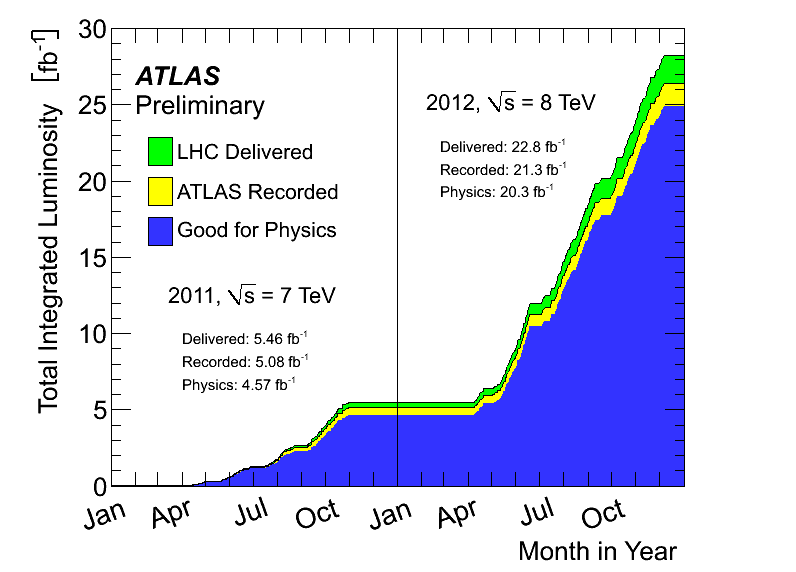
\includegraphics[width=0.48\textwidth]{intlumivstime2011-2012DQ.png}}
  \subfigure[Mean number of interactions per bunch crossing]{\label{fig:mu_2011_20112} 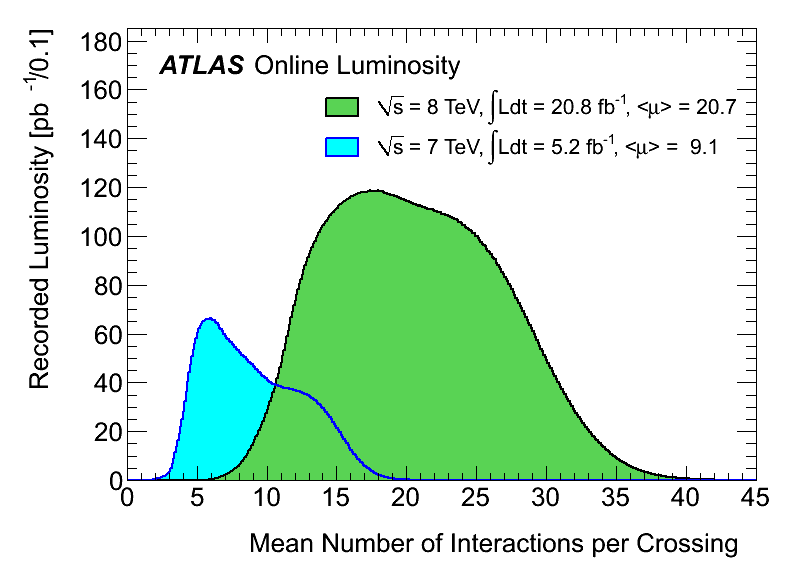
\includegraphics[width=0.48\textwidth]{mu_2011_2012-nov.png}}\\
\caption{(a): luminosity delivered and recorded in ATLAS. (b): mean number of interaction per bunch crossing in 2011 and 2012 data \cite{twiki_lumi}.}
\label{fig:intlumi_atlas}
\end{figure}
